\section{The Interface}
Next, we will describe the components of the \sys interface used in this demonstration. 

\begin{figure}[t]
\centering
 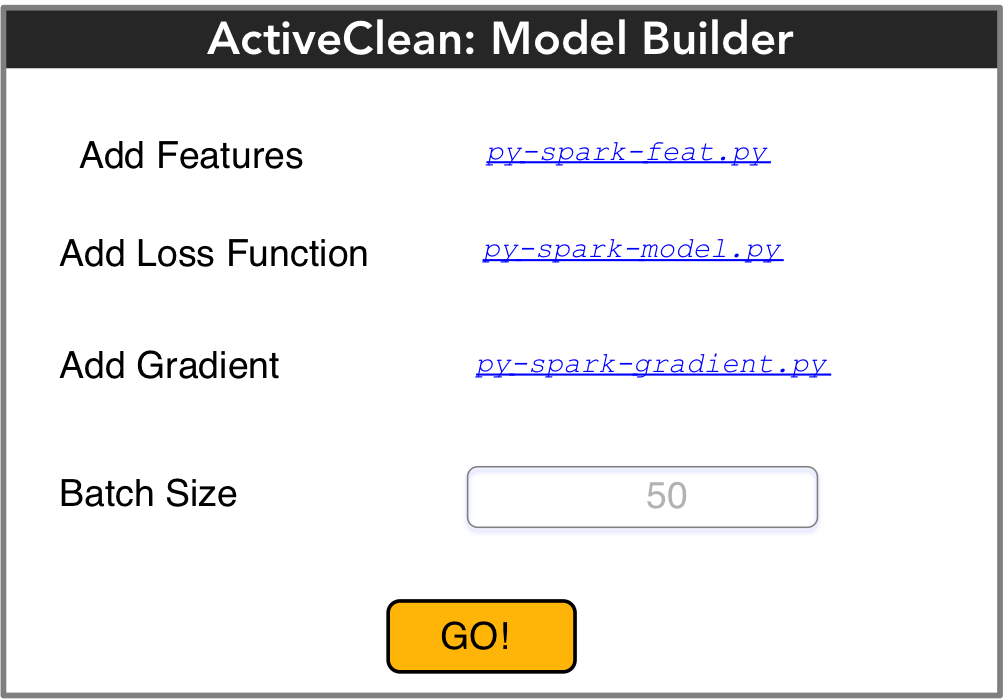
\includegraphics[width=0.48\columnwidth]{figs/interface1.png}
 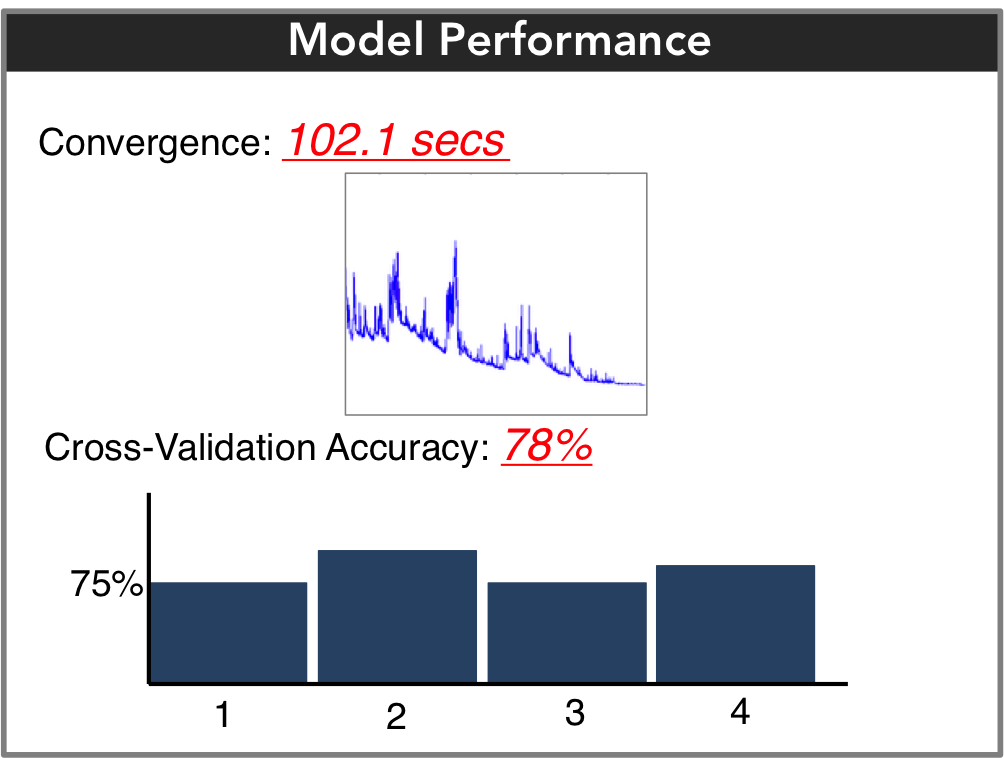
\includegraphics[width=0.48\columnwidth]{figs/interface2.png}
 \caption{Initialization. The analyst loads user-defined model functions into \sys and then trains an initial model on the dirty data \label{irun}}
\end{figure}

\subsection{Initialization}
The analyst first uses the \textsf{Model Builder} (Figure~\ref{irun}, left panel) to specify and initialized the problem.
She loads three user-defined functions written in PySpark~\cite{pyspark} based on the descriptions in the previous section, and
optionally  tune the stopping criteria.
Once the model is trained, the right panel will show summary information.
The top shows \textsf{Performance} information, and plots the model's convergence as a function of iteration,
The bottom shows model accuracy information, and shows the cross-validation accuracy if it is a classification task and the hold-out residual error if it is a regression task.

\subsection{Diagnose Interface}
Suppose the analyst is unhappy with her model, and wishes to understand why her prediction accuracy is poor.
She can then open the \textsf{Diagnose} panel to understand why (Figure~\ref{diag}).
When she opens the \textsf{Diagnose} panel, \sys applies the importance sampling algorithm to select and visualize a subset of examples from the dataset.
Since these points are in general high dimensional, we apply T-SNE~\cite{van2008visualizing},
a non-linear dimensionality reduction technique that is widely used to visualize complex data distributions,
to visualize the points in a 2-D plot.
%The batch size setting controls the number of examples plotted on this screen.
The points are color coded to indicate the label in the case of classification.
The analyst can select examples from the plot for further inspection.

\begin{figure}[t]
\centering
 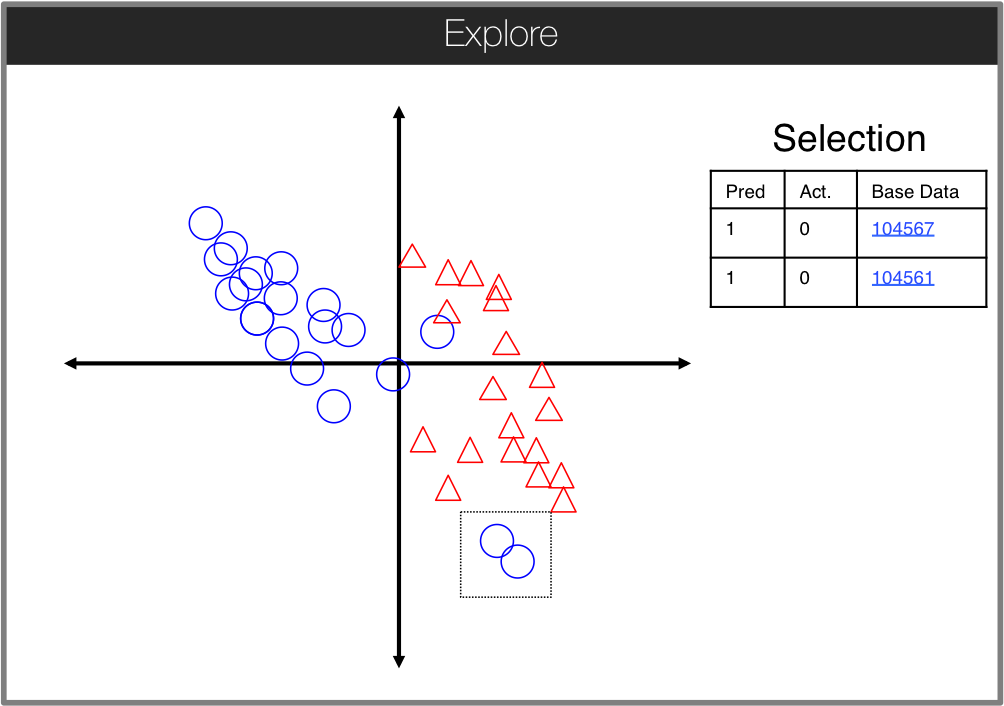
\includegraphics[width=0.5\columnwidth]{figs/interface3.png}
 \caption{The diagnose inteface. The analyst can select and inspect suspect data. \label{diag}}
\end{figure}

\subsection{Cleaning Interface}
If the analyst decides that the data are actually dirty, then she can open the \textsf{Clean} panel.
This panel gives her the option to remove the dirty record, apply a custom cleaning operation (specified in Python), or pick from a pre-defined list of cleaning functions.
% \sys keeps track of previously written cleaning operations and the analyst need not write a new script each time, and simply assign a previously written transformation. 
Custom cleaning operations are added to the library to help taxonomize different types of errors and reduce analyst cleaning effort.
%This serves two purposes: (1) it reduces effort for the analyst, and (2) it helps \sys taxonomize the types of errors in the dataset.
This also provides a hint about which data are similarly corrupted (and thus fixed), we can guide future samples to draw similar data in future samples.
We do this by training a classifier to learn the conditions for when the operation is applicable to a record, the details are described in our technical report~\cite{activecleanarxiv}.

\begin{figure}[t]
\centering
 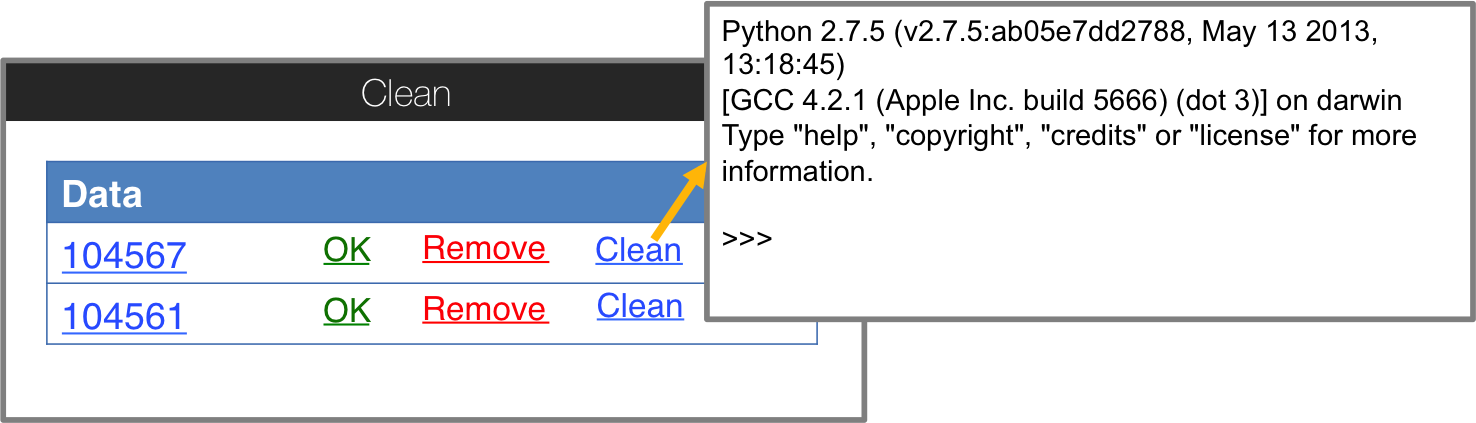
\includegraphics[width=\columnwidth]{figs/interface4.png}
 \caption{Cleaning Interface. The analyst can choose to remove data, write a custom cleaning operation, or automatically clean the data using an existing cleaning operation.}
\end{figure}

\subsection{Iteration and Updates}
Finally, after the data sample is cleaned, \sys updates the current best model, and re-runs the cross-validation to visualize changes in the model accuracy (Figure~\ref{modelacc}).
At this point, \sys begins a new iteration by drawing a new sampling of records to show the analyst.  
Once \sys satisfies the stopping conditions, the current best model parameters along with the (partially) cleaned dataset are returned to the analyst.


\begin{figure}[t]
\centering
 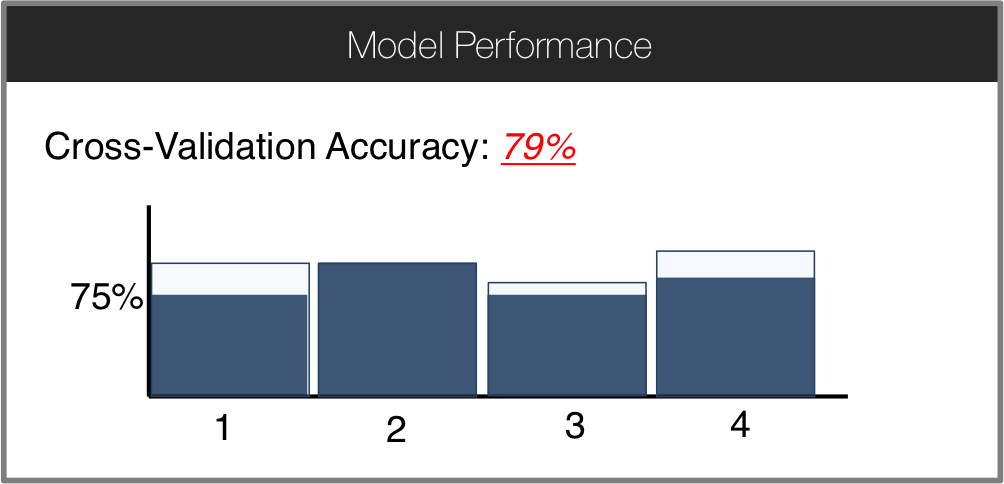
\includegraphics[width=0.4\columnwidth]{figs/interface5.png}
 \caption{Update Visualization. We visualize the changes in model accuracy after data cleaning.}\label{modelacc}
\end{figure}